\section{Groupchat}
\label{sec:groupchat}

The developed system is based on a client/server architecture, which uses a many-to-many relationship. The program enables multiple clients to communicate with multiple servers. Besides replicated and distributed storage service, with the created extension clients are now able to exchange messages with each other.\\ In the following sections the functionalities of the groupchat is described by first representing newly added commands to the client library and then explaining the execution of the workflow. \\
The main goal here is to clarify the usage of the system for a client, who does not have the full knowledge of how a distributed database system works.

\subsection{New Commands for the Groupchat}
\label{sec:groupchat_commands}

In addition to already implemented commands, such as "put" or "get" with the purpose of accessing the database or commands like "logLevel" for changing the level of the logs dynamically, seven more commands are implemented in order to realise the groupchat extension.\\
Following commands are possible during a chat session:
\begin{enumerate}
  \item 	PUT <key> <value>: \\
Stores the given value and allows future access to it through the provided key. 
  \item PUT <key>:\\
Deletes the value assigned to the given key.
  \item GET{<key>}:\\
Inserts the value assigned to the given key into the message.
  \item WSP <user1>,..,<userN> <msg>:\\
Sends a whisper to the users provided by the client. It is possible for a chatroom to have     up to 30 clients in it. The logic behind whispering feature is a client should be able to send messages during a chat session, only to the people who he/she wants to share it with.  
  \item QUIT:\\
  Leaves the chat session.
  \item ACTIVE:\\
   Returns a list of all users in the chatroom. A client does not have to always keep up with the notifications about who joined the chat or left it, that is why the command "ACTIVE" eases for a client to see online members at that moment.
  \item HELP:\\
  Displays the help text.
\end{enumerate}
Put and delete operations are fulfilled with the help of a chatbot. Most of the software systems include a chatbot in their system to work as a costumer service. Our intention by implementing a chatbot is to decrease the workload of the chatroom.

\subsection{Chatbot}
\label{sec:groupchat_chatbot}
One of the extensions followed by the groupchat is a chatbot which is designed to help chatrooms to access the distributed database. The chatbot shares a lot of similarities with the client application. When a client wants to perform read or write operations while chatting, requests are directed to the chatbot.


\subsection{Execution of the Workflow}
\label{sec:groupchat_executionoftheworkflow}

To start off, in the same sense as Milestone 4, initially the External Configuration Service (ECS), where the storage servers are monitored and controlled, is executed. Following that, depending on client's decision, a number of servers are created. A client must connect to one of the servers by typing its IP address and port number in order to use the database system.

\subsubsection{Unique Username}
\label{sec:groupchat_executionoftheworkflow_uniqueusername}
After successfully connecting to a key-value server, the client has to either enter a username or use the command QUIT to have a username randomly assigned to him. Usernames are implemented as globally unique identifiers for the clients, which prevents different clients from having the same username in different chatrooms. That way users are guaranteed to know who they are communicating with as long as their partner is connected to the system. 

In order to avoid unnecessary extra connections, the ECS stores a list of users. Whenever a client tries to set its username, the request gets sent through the server to the ECS, which then checks if the username has been already taken by a client connected to any of the servers online. The end user either receives a welcome message with the username displayed if the operation was succesful, or an error message otherwise.
 
\subsubsection{Chat Command}
\label{sec:groupchat_executionoftheworkflow_chatcommand}

Moreover, to use the chatroom client needs to type “chat” on the console and choose a chatID for the chatroom and type it right next to the command “chat”. A chatroom is created with the given id, subsequently client have two options: either enter a private room with a password feature or a public room. 
\subsubsection{Private/Public Chatrooms}
\label{sec:groupchat_executionoftheworkflow_chatrooms}

If the client is the first person to create a private chatroom, then the right to give a password to the room belongs to the same person.
\subsubsection{Password}
\label{sec:groupchat_executionoftheworkflow_chatrooms_password}

Another client who is connected to the same server and wants to chat in the same chatroom can only access to the private room with the selected password by the client, who created the private chatroom. The password is hashed in order to provide safety for the client. If client wants to have a public chatroom, then a password is not needed.\\
\\
To prevent heavy workload for a server, a chatroom has the maximum capacity of 30 people. The chatroom offers a communication platform for all the clients sharing the same chatroom. Every message sent by the clients have timestamps in order to keep on track with the flow of the messages for other clients. One message can contain maximum 200 characters.\\
When a client joins a chatroom, all the messages which sent until that time, will be visible to the latest joined client and all the members will be informed about who joined or left the chatroom. 
\subsubsection{Saved Messages}
\label{sec:groupchat_executionoftheworkflow_savedmessages}

The messages are saved into a .txt file under the directory of the respective server.\\

Whenever a client wants to leave the chatroom, QUIT can be typed in order to use the functionalities of replicated and distributed database service from Milestone 4. To enable the chatroom service client only needs to enter “chat” command with the desired chatID. 

\begin{figure}[h]
	\centering
	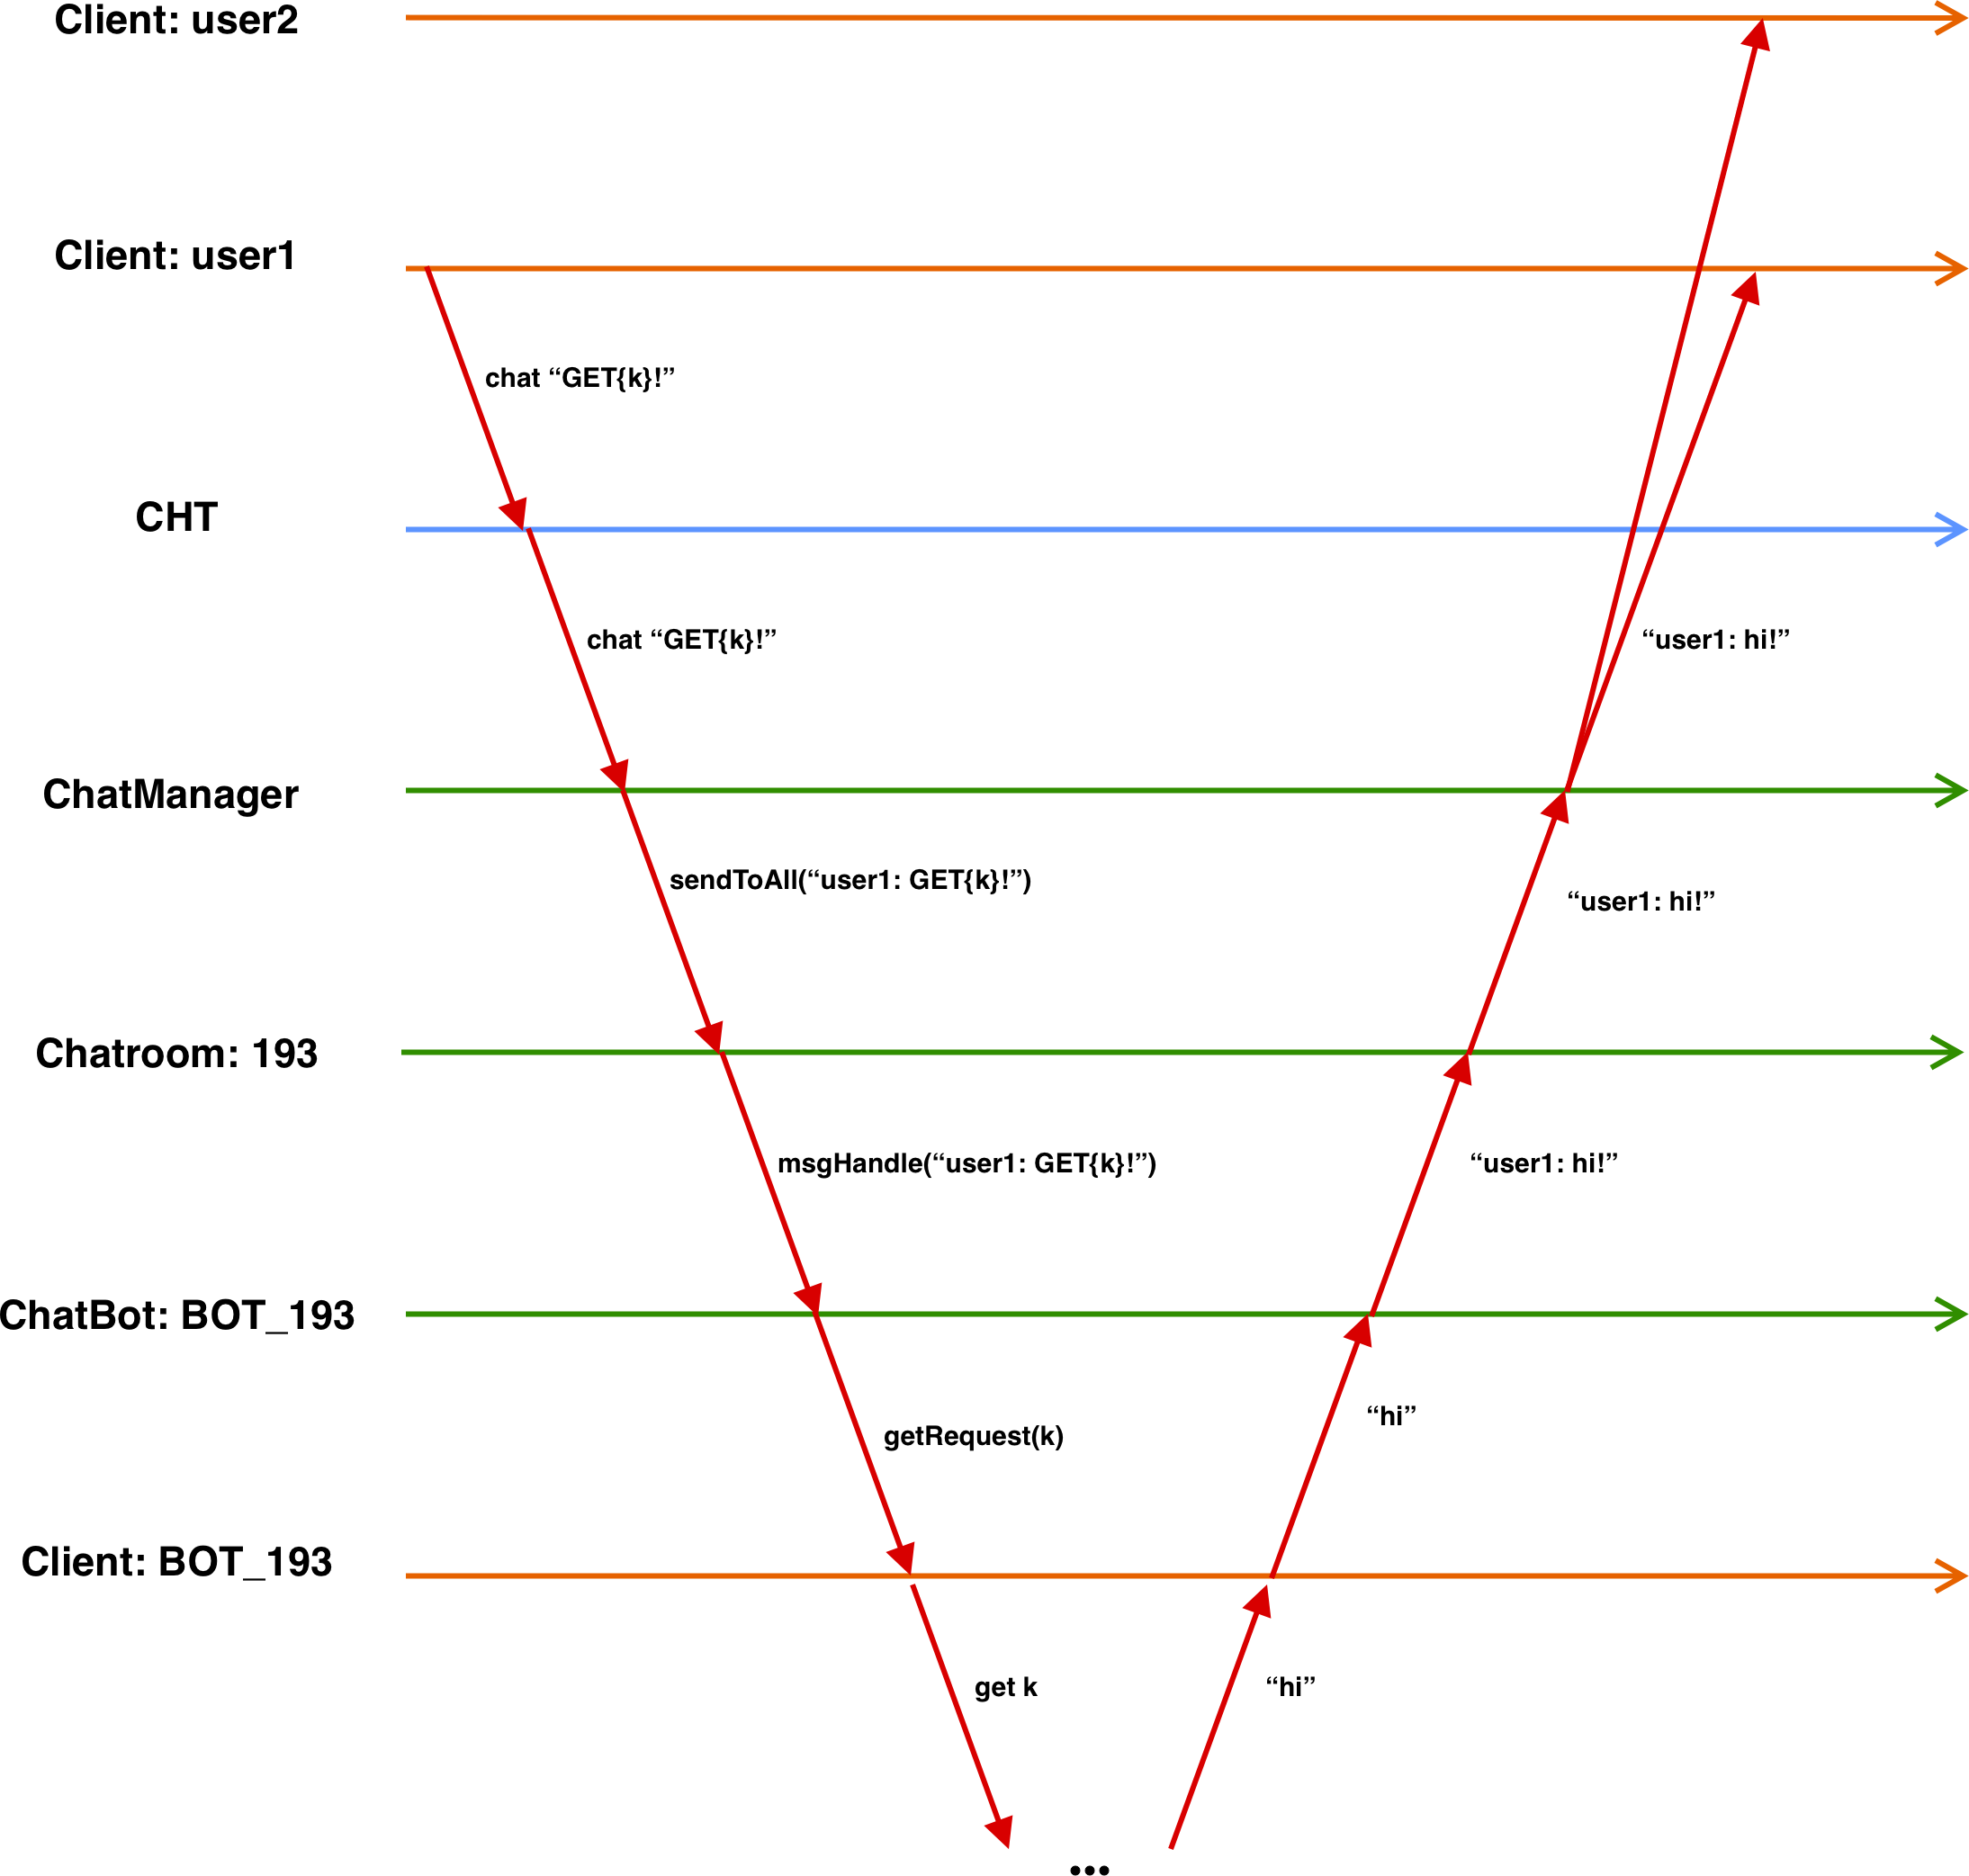
\includegraphics[width=\linewidth]{figures/chat_graph.png}
	\caption{Client side architecture}
\end{figure}



